Para o experimento de avaliação do desempenho do plano de dados do núcleo da rede 5G, foi executada, por 60 s, a ferramenta \textit{iPerf} 2.0 simultaneamente em cada UE conectado ao núcleo 5G.
Em um primeiro momento, foi utilizada a máquina virtual em sua configuração máxima, com 12 núcleos virtuais de CPU e 8 GB de memória RAM.
Após a coleta e o processamento dos dados gerados pela ferramenta \textit{iPerf}, foram gerados os gráficos representando a largura de banda por segundo dos núcleos de rede 5G \textit{free5GC} e \textit{Open5GS} testados.

A Figura \ref{fig:exp2_free5gc_12-8} apresenta os gráficos com a largura de banda para cada configuração de quantidade de UE para o núcleo \textit{free5GC} na máquina virtual com 12 núcleos virtual de processador e 8 GB de memória RAM.

\begin{figure}[H]
    \centering
    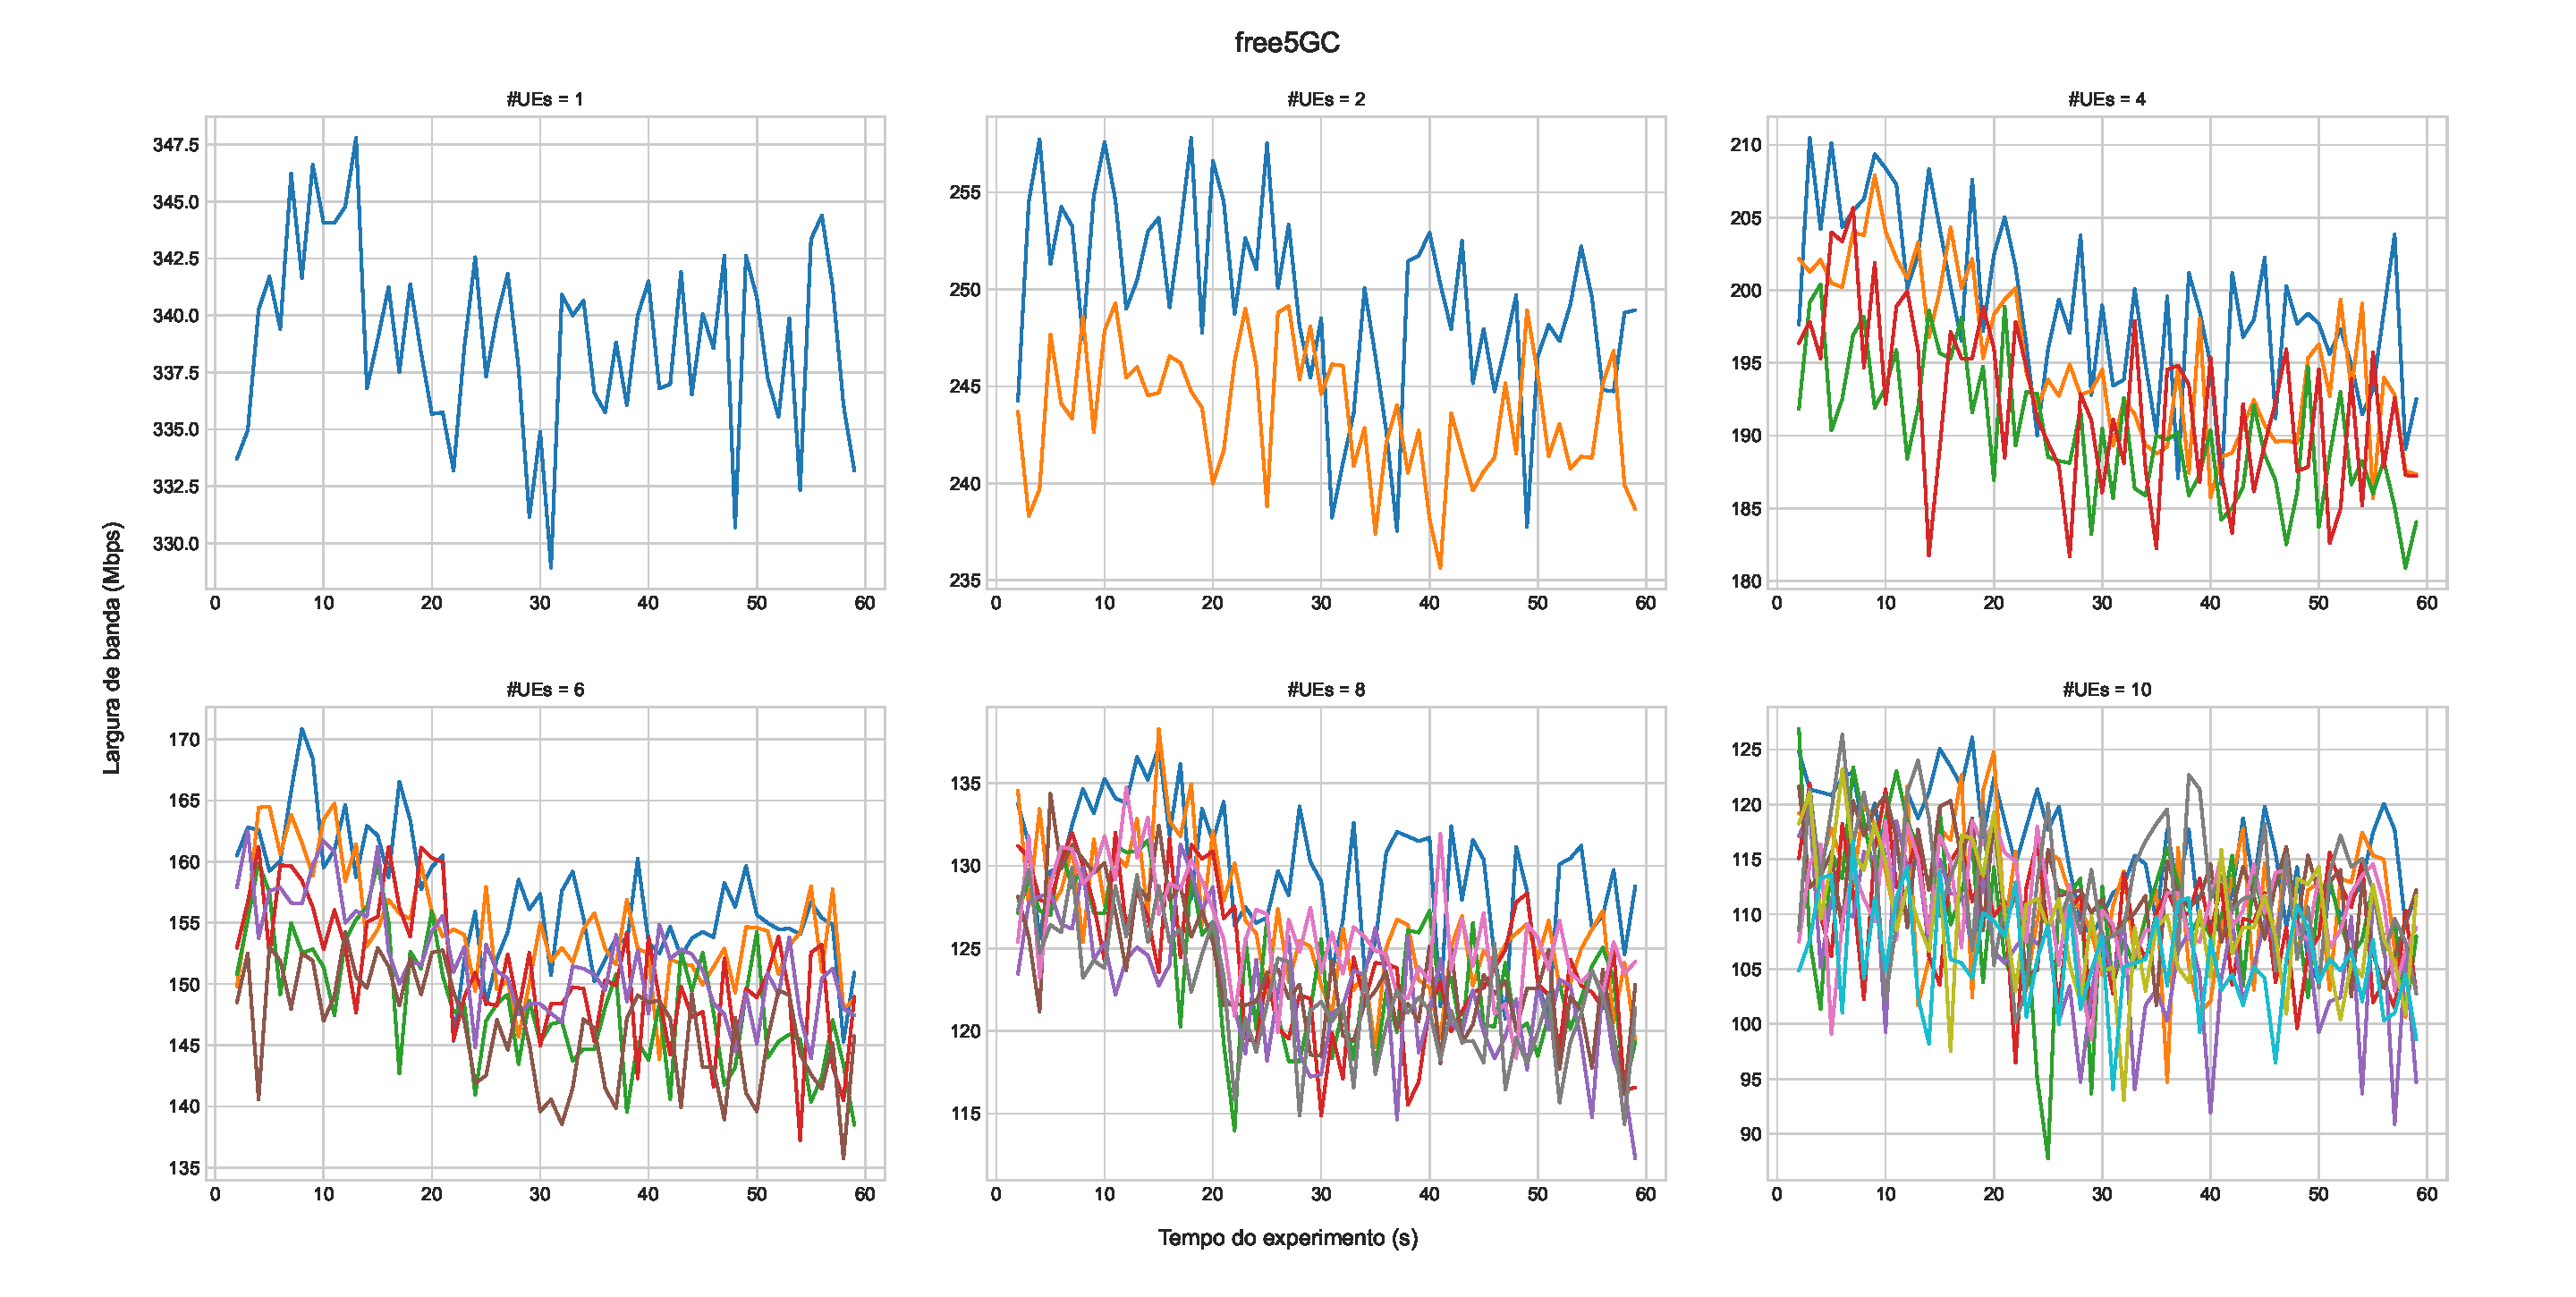
\includegraphics[width=1\textwidth]{TG2/Chapters/DataAnalysis/Figures/EXP2-free5GC-12C-8GB.pdf}
    \caption{Largura de banda para cada configuração de quantidade de UE para o núcleo \textit{free5GC}}
    \label{fig:exp2_free5gc_12-8}
\end{figure}

A Figura \ref{fig:exp2_open5gs_12-8} apresenta os gráficos com a largura de banda para cada configuração de quantidade de UE para o núcleo \textit{Open5GS} na máquina virtual com 12 núcleos virtual de processador e 8 GB de memória RAM.

\begin{figure}[H]
    \centering
    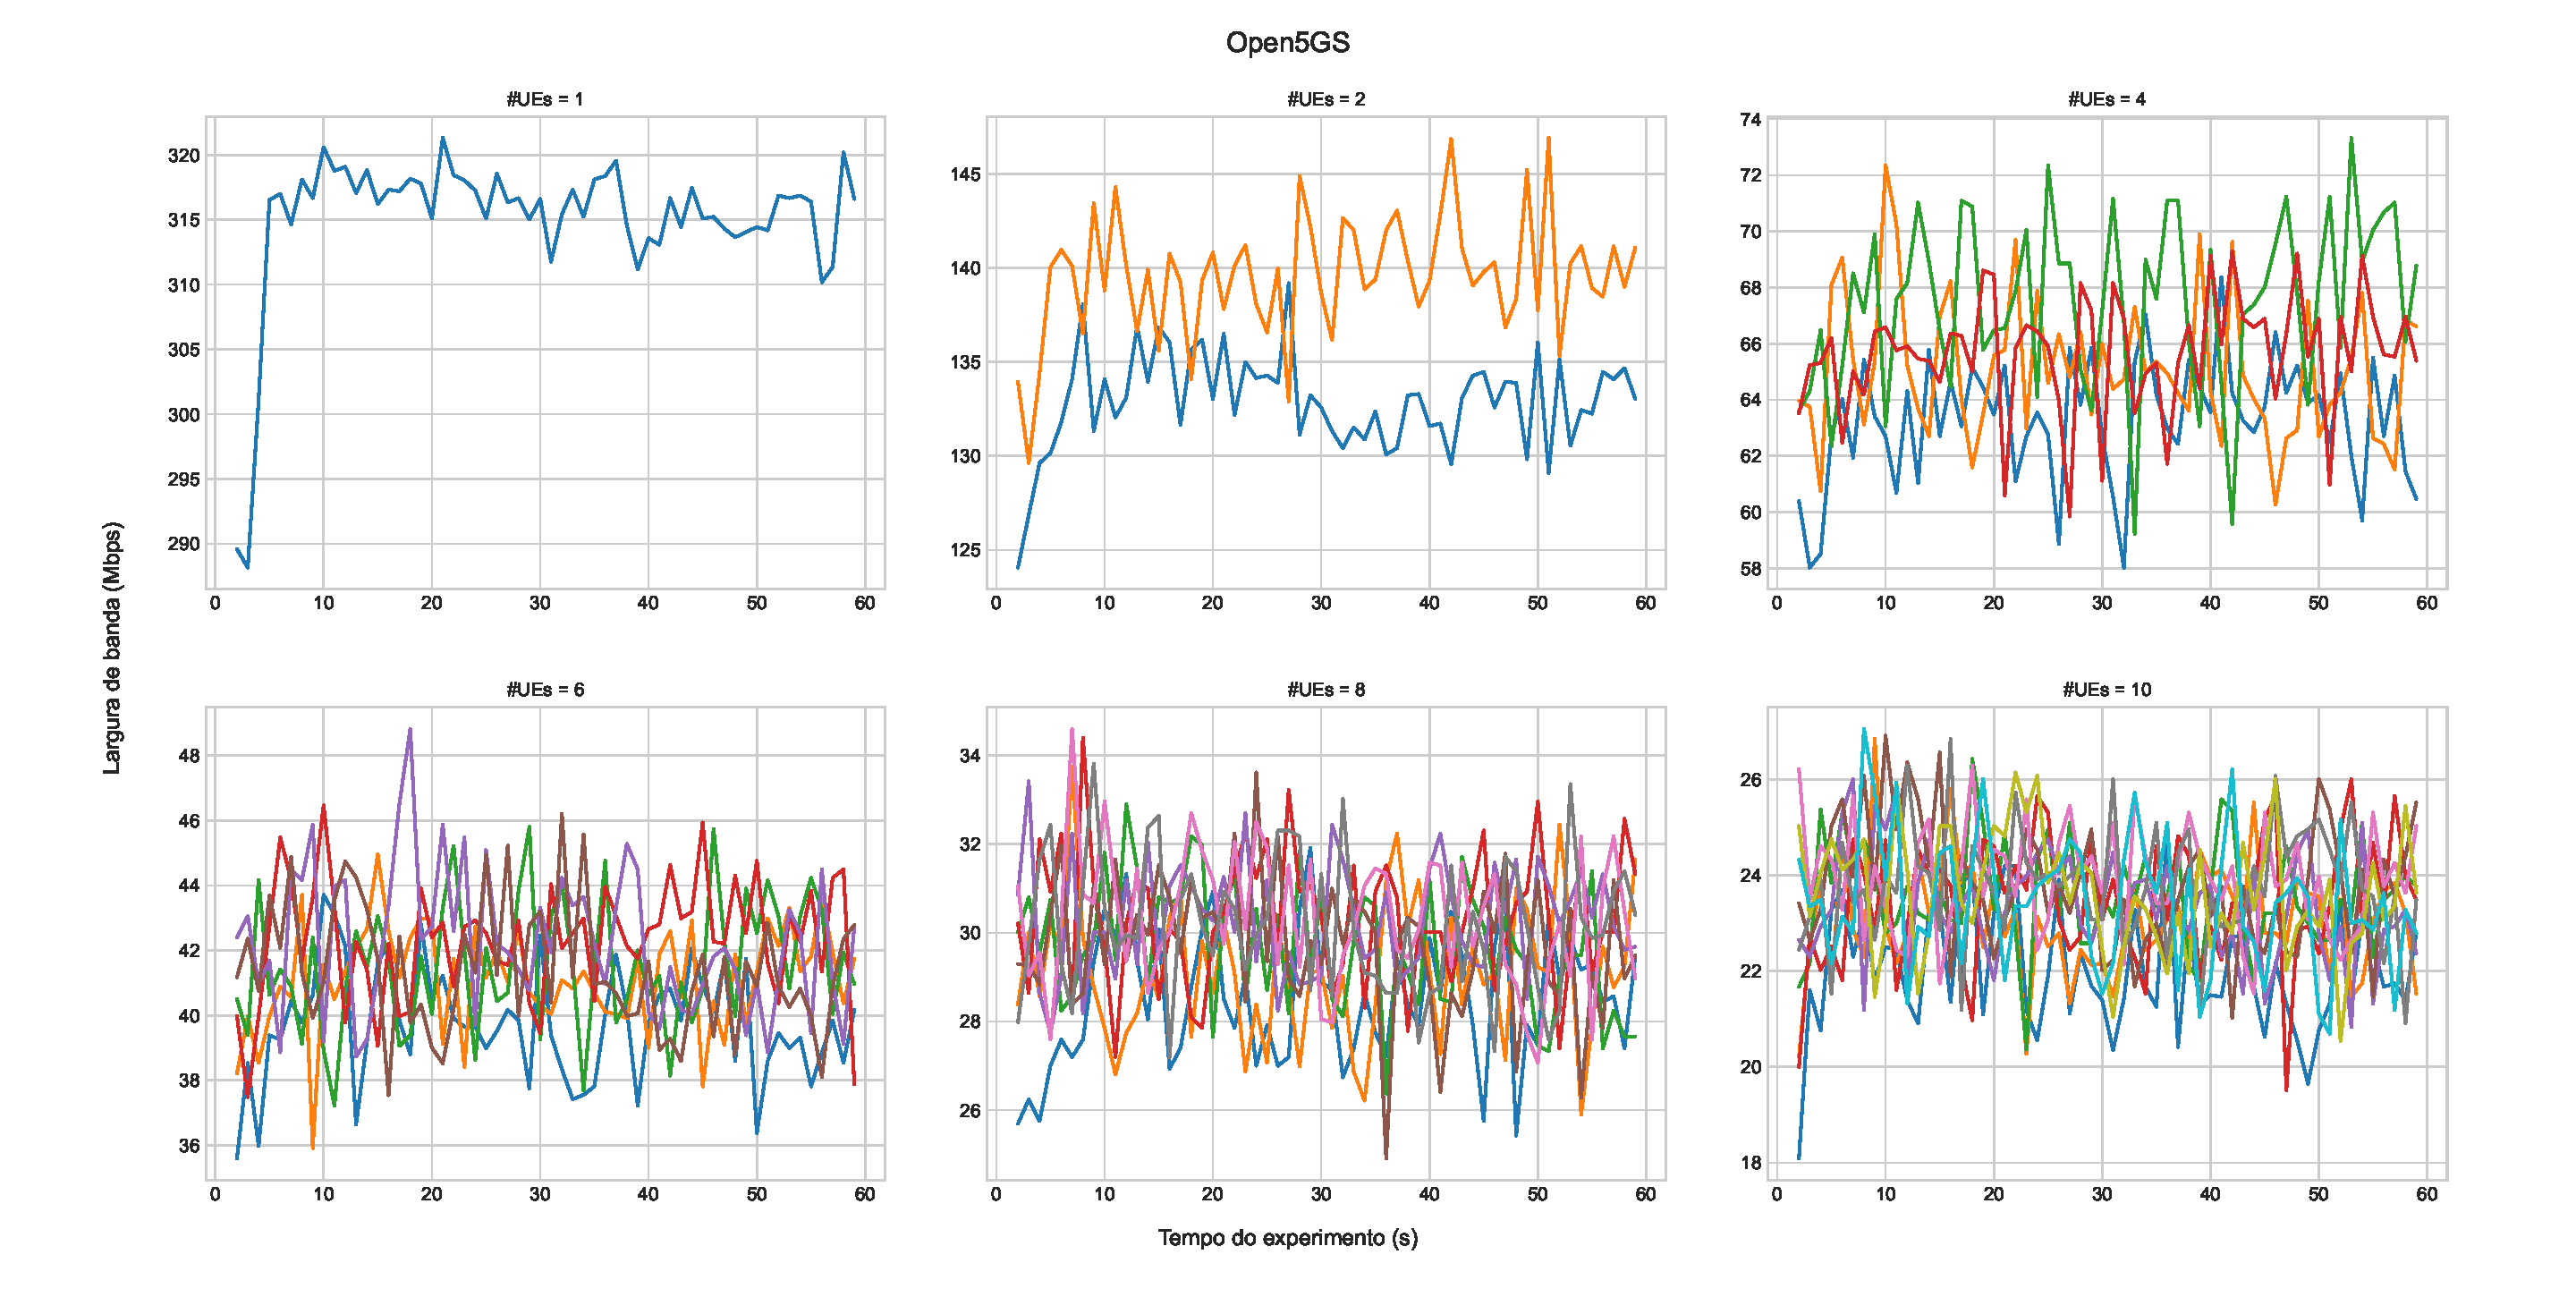
\includegraphics[width=1\textwidth]{TG2/Chapters/DataAnalysis/Figures/EXP2-Open5GS-12C-8GB.pdf}
    \caption{Largura de banda para cada configuração de quantidade de UE para o núcleo \textit{Open5GS}}
    \label{fig:exp2_open5gs_12-8}
\end{figure}

Através desses gráficos, é possível observar que a largura de banda disponível para os UEs não é estável, oscilando durante toda a execução do experimento.
Para uma melhor visualização dos valores agregados de cada execução desse experimento, foram criados gráficos de barra.
O eixo X do gráfico representa o número de UEs em cada rodada do experimento, onde segmento da barra representa o UE de mesma cor das duas figuras anteriores.
Cada barra do gráfico representa a largura de banda média em Mbps agregada entre os UEs.
A Figura \ref{fig:exp2_all_12-8} apresenta o valor agregado da largura de banda para cada configuração de quantidade de UE para a máquina virtual com 12 núcleos virtuais e 8 GB de memória RAM.

\begin{figure}[H]
    \centering
    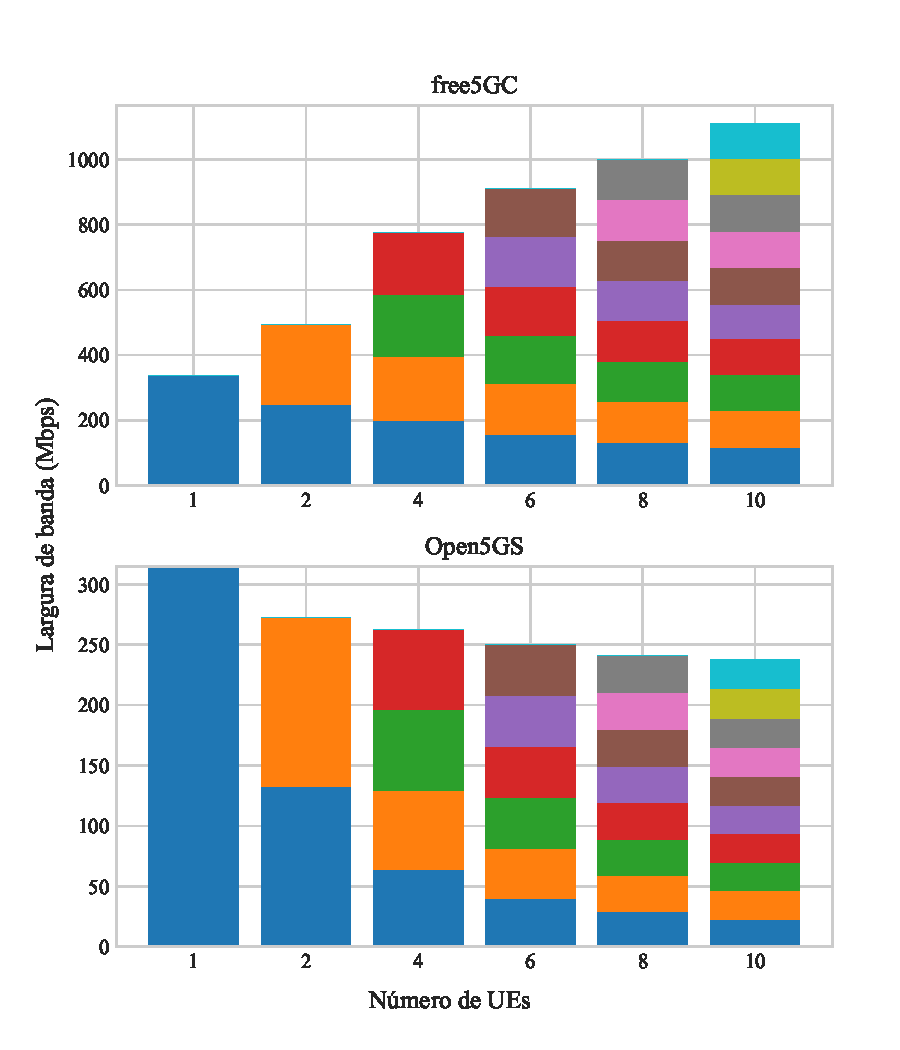
\includegraphics[width=1\textwidth]{TG2/Chapters/DataAnalysis/Figures/EXP2-ALL-12C-8GB.pdf}
    \caption{Valor agregado da largura de banda para cada configuração de quantidade de UEs}
    \label{fig:exp2_all_12-8}
\end{figure}

Nesse experimento, percebe-se que no núcleo \textit{free5GC} a largura de banda total entre cada execução aumenta de acordo com a quantidade de UEs conectados.
O valor médio de largura de banda para esse núcleo com um UE conectado é de 338.4 Mbps, aumentando para 777.0 Mbps com quatro UEs conectadas e 1109.9 Mbps com 10 UEs conectadas.
Em contrapartida, o comportamento do núcleo \textit{Open5GS} se opõe ao \textit{free5GC}. No núcleo \textit{Open5GS}, o valor médio da largura de banda para um UE conectado é de 314.5 Mbps, reduzindo para 262.7 Mbps com 4 UEs conectadas e 237.9 Mbps ao conectar 10 UEs simultâneas.
Esse experimento demonstra que o núcleo \textit{free5GC} possui melhor estrutura para gerenciar o tráfego de dados de UEs em escala em relação ao núcleo \textit{Open5GS}.

Ao limitar a quantidade de recursos disponíveis para a execução do experimento, diminuindo a quantidade de núcleos virtuais de processador e memória RAM da máquina virtual, percebe-se que o desempenho do plano de dados para o núcleo \textit{free5GC} é diretamente proporcional à quantidade de núcleos virtuais disponíveis.
A Figura \ref{fig:exp2_all_8-8} representa o desempenho médio agregado do plano de dados para a execução do experimento em uma máquina virtual com 8 núcleos virtuais de processador e 8 GB de memória RAM.
Nesse caso, largura de banda máxima do plano de dados para o núcleo \textit{free5GC} é reduzida para 1004.2 Mbps quando executado com dez UEs simultâneos.
Essa redução de desempenho pode ser explicada devido à limitação na carga máxima de processamento suportada pela máquina virtual.

\begin{figure}[H]
    \centering
    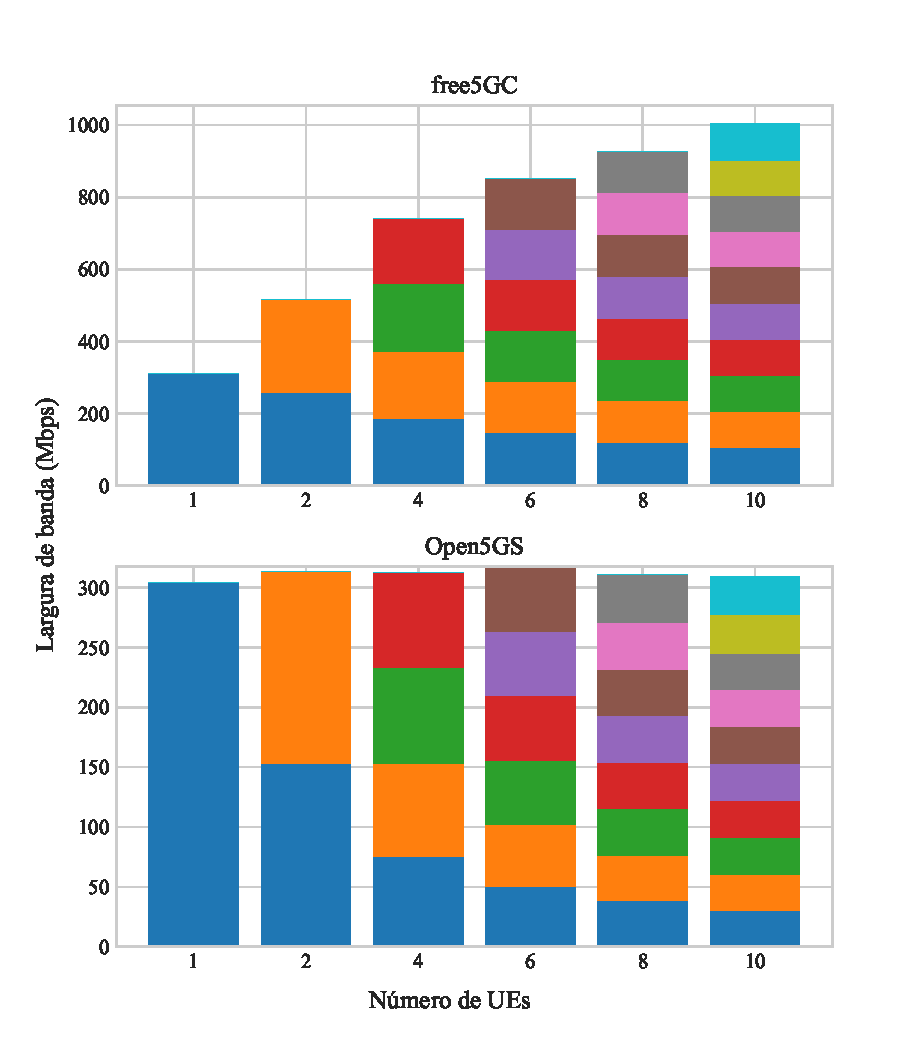
\includegraphics[width=1\textwidth]{TG2/Chapters/DataAnalysis/Figures/EXP2-ALL-8C-8GB.pdf}
    \caption{Valor agregado da largura de banda para cada configuração de quantidade de UEs}
    \label{fig:exp2_all_8-8}
\end{figure}

A redução de desempenho do plano de dados fica mais visível ao limitar-se ainda mais a quantidade de núcleos virtuais disponíveis para o experimento.
Na Figura \ref{fig:exp2_all_6-8}, onde a máquina virtual é executada com 6 núcleos virtuais de processador e 8 GB de memória RAM, é possível perceber que o desempenho máximo do plano de dados do núcleo \textit{free5GC} é atingido com seis UEs simultâneos.

\begin{figure}[H]
    \centering
    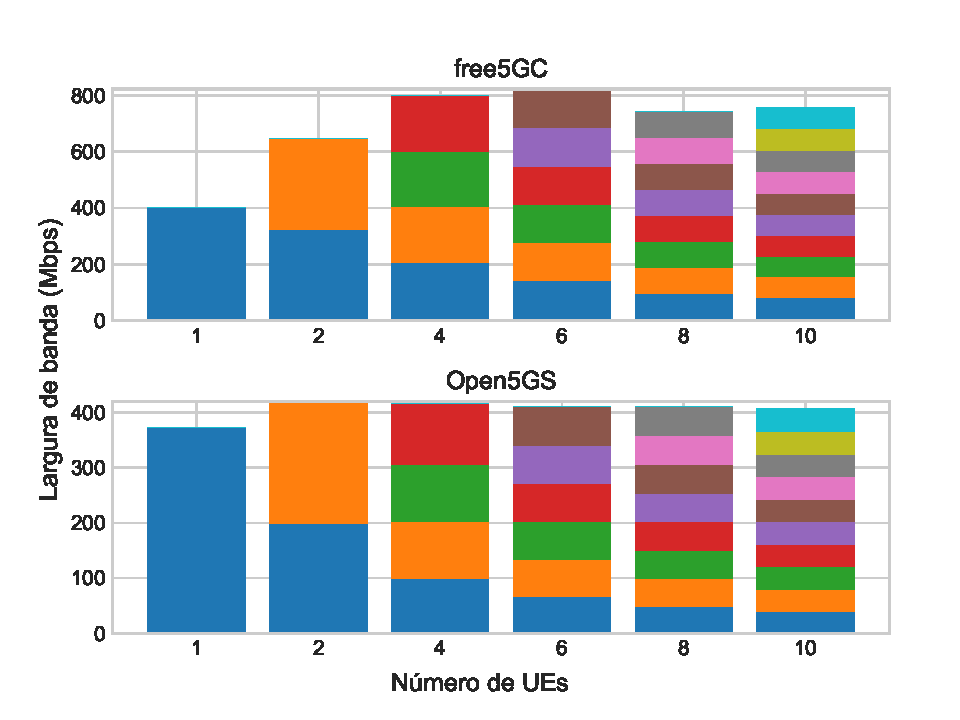
\includegraphics[width=1\textwidth]{TG2/Chapters/DataAnalysis/Figures/EXP2-ALL-6C-8GB.pdf}
    \caption{Valor agregado da largura de banda para cada configuração de quantidade de UEs}
    \label{fig:exp2_all_6-8}
\end{figure}

A Figura \ref{fig:exp2_all_4-4} representa os resultados obtidos para a execução do experimento em uma máquina virtual com 4 núcleos virtuais de processador e 4 GB de memória RAM.
Essa configuração foi utilizada para simular um cenário com recursos limitados.
Neste caso, o desempenho máximo do núcleo \textit{free5GC} ocorre com quatro UEs simultâneos. 
A redução de desempenho para testes com maior quantidade de UEs simultâneos é explicada pela sobrecarga de uso de processador causada pela quantidade de UEs trafegando dados em paralelo.
Os detalhes de uso de recursos são apresentados na Seção \ref{sec:results-resource-analysis}.

\begin{figure}[H]
    \centering
    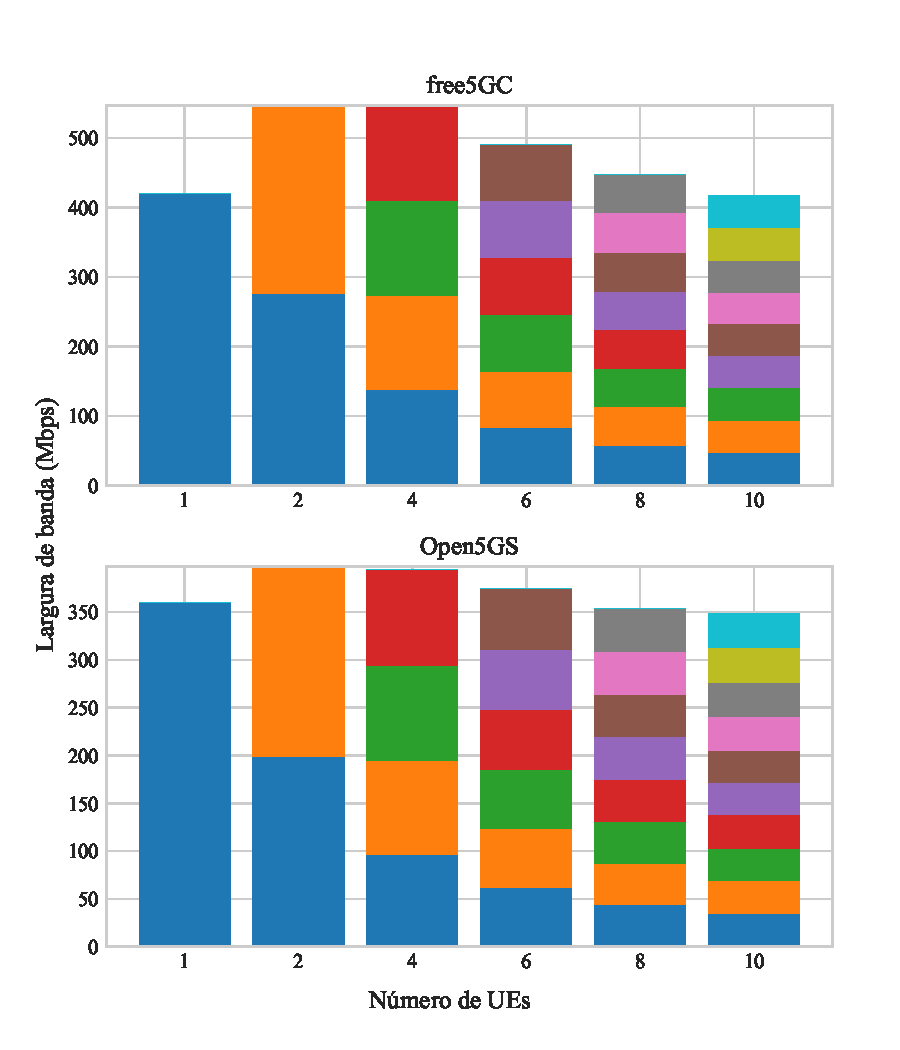
\includegraphics[width=1\textwidth]{TG2/Chapters/DataAnalysis/Figures/EXP2-ALL-4C-4GB.pdf}
    \caption{Valor agregado da largura de banda para cada configuração de quantidade de UEs}
    \label{fig:exp2_all_4-4}
\end{figure}
